\section{Tuesday, February 20th}
\subsection{Reading and Quiz Announcements}
\begin{itemize}
    \item Reading: Shannon 3, finish T\&C Ch. 2.
    \item Quiz 3 this Thursday on differential entropy.
    \item Project Part 3 released tonight.
\end{itemize}

\subsection{Goals}
Finish up Differential Entropy.

\subsection{Last Class Recap}
Last class we left off with the following argument: We tried to make three axioms corresponding to the discrete case:
\begin{enumerate}
    \item Continuity: \( h \) is continuous. \( z^{\Delta x} \) i.i.d.\ converges to \( f_X \) as \( \Delta x \to 0 \).
    \item Extrinsic: If \( X \sim \text{Unif}[\mathcal{X}] \), then \( h[X] = \log(|\mathcal{X}|) \).
    \item Chain Rule.
\end{enumerate}
Thus, \( h[X] \) as \( \Delta x \to 0 \) approximately equals \( h[z^{\Delta x}] \) which equals \( H[Y^{\Delta x}] + \mathbb{E}_y[h[z^{\Delta x} | Y^{\Delta x} = y]] \) and equals \( H[Y^{\Delta x}] + \mathbb{E}_{Y^{\Delta x}}[\log(\Delta x(Y))] \), which by Riemann integration, is approximately \( -\int_{\mathcal{X}} f_X(x) \log(f_X(x)) \, dx \) and equals \( -\mathbb{E}_X[\log(f_X(x))] \) (the expected surprise).

Where the uncertainty in which bin contains \( x \) equals the number of bins, and the uncertainty in \( z^{\Delta x} \) given the bin approximates the uncertainty left over in \( X \) given \( Y^{\Delta x} \), as we refine to higher precision/resolution.

We are matching relative entropies in the limit...
% \begin{flalign*}
% \text{If } |\mathcal{X}| \text{ is finite then } \Delta x = \frac{|\mathcal{X}|}{|y|}
% \text{. If we accept the second axiom, then}
% h[X] - h[\text{uniform } |\mathcal{X}|] \xrightarrow{\simeq}{\Delta x \to 0} H[Y^{\Delta x}] - H[\text{uniform on } |y^{\Delta x}|]
% D(f_x || \text{Uni}[\mathcal{X}]) \xrightarrow{\simeq}{\Delta x \to 0} D(p_{\Delta x} || \text{Uni}[y^{\Delta x}])
% \text{. Match these ideas relative to a reference uncertainty.}

% \text{Goal: derive (2.) from (3.) — axioms above:}
% \text{We start with } X \sim \text{Uni}[\mathcal{X}] \text{ since our second axiom is claiming something about Uniform distribution.}
% \text{To use the chain rule, we need another r.v. So let us partition } \mathcal{X} \text{ into } n \text{ sets, each of size } \Delta x = \frac{|\mathcal{X}|}{n}
% \text{. Let } Y \text{ be the indicator for the bin. Now we are ready to use the chain rule:}
% h_d[X] = h_d[X, Y] \text{ since one r.v. determines all info about the other.}
%          = H[Y] + h[X | Y]
%          = H[Y] + \mathbb{E}_y[h[X | Y=y]] 
%          = \log_d(n) + \mathbb{E}_y[h[\text{Uni}[\frac{|\mathcal{X}|}{n}]]]
%          = \log_d(n) + h[\text{Uni}[\frac{|\mathcal{X}|}{n}]] \text{ since we don't depend on the expectation.}
%          = \log_d(n) + h_d[\text{Uni}[{|\mathcal{X}|}]] - \log_d(n) \text{ for all } n, |\mathcal{X}| \text{ since } 
% h_d[\text{Uni}[{|\mathcal{X}|}]] = h[\text{Uni}[\frac{|\mathcal{X}|}{n}]] + \log_d(n)

% u_d[\mathcal{X}] - u_d(\frac{\mathcal{X}}{n}) = \log_d(n) \text{ but this is only defined up to difference so we need to pick a reference.}
% \text{We choose: } u_d(\Delta x) = 0
% \text{. Then } u_d(n \Delta x) = \log_d(n)
% h_d[\text{Uni}[\mathcal{X}]] = \log_d(|\mathcal{X}|) - \log_d(\Delta x) \text{, where } \Delta x = \frac{\mathcal{X}}{n}

% \text{Usually, } \Delta x = 1 \text{ naturally (it was hiding in this construction) as this gives us } \log_d(1) = 0
% \text{. Even if we don't specify it, this leads to properties that we do not see in the discrete entropy.}
% \end{flalign*}

% 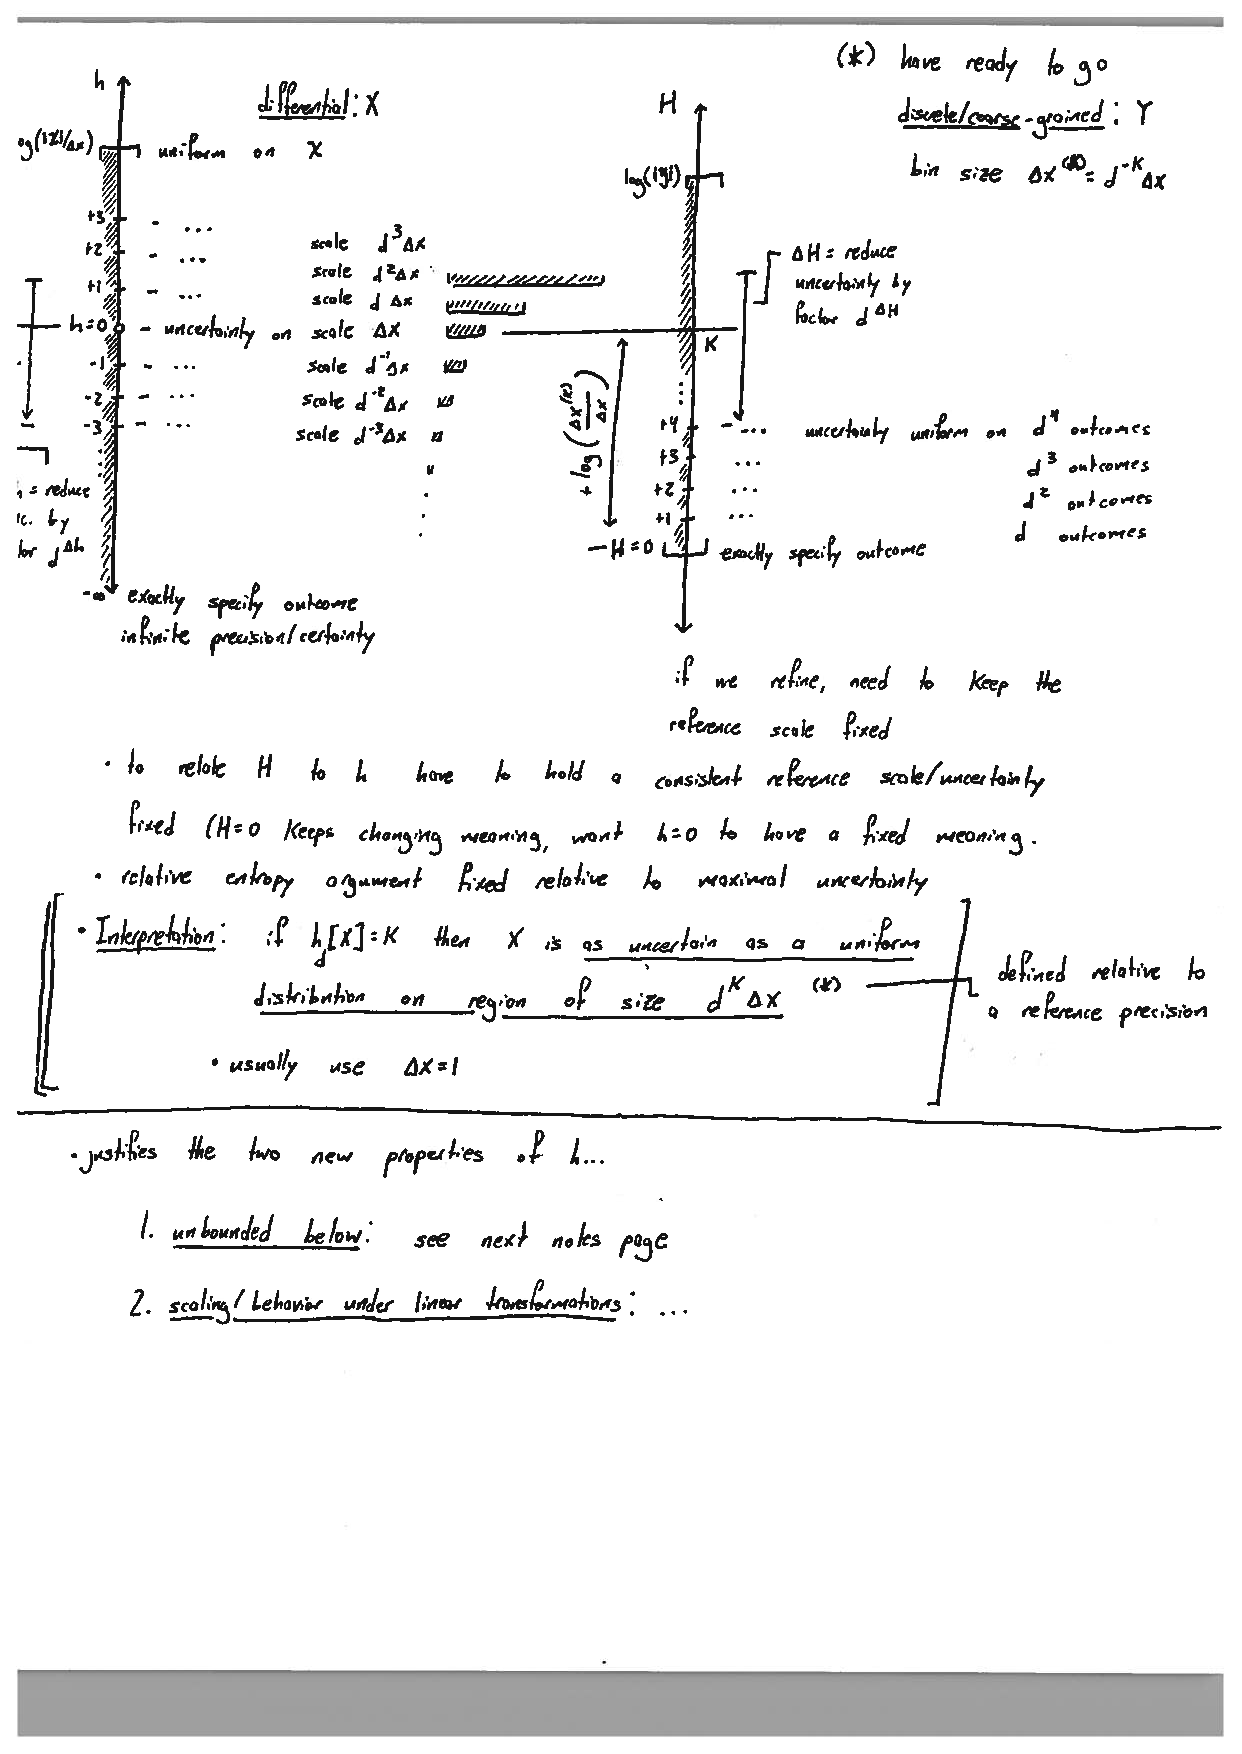
\includepdf[scale=1]{img/Differential_vs_Discrete_schematic.pdf}

% \begin{flalign*}

% \text{Negative relative entropy means we are more certain than our reference scale.}

% \text{If our relative entropy is } -\infty \text{ then we are infinitely more certain than our reference scale (we have exactly specified outcome to infinite precision).}
% \end{flalign*}

\hrulefill

\subsection{Properties of Differential Entropy}
Properties of Differential Entropy that are not shared by discrete entropy:
\begin{enumerate}
    \item Unbounded below: For \( X \sim p \), \( X \in \mathcal{X} \), and \( |\mathcal{X}| \), let \( p = \text{Uni}(|S|) \), then \( h_d[X] = \log_d(|S|) \to -\infty \) as \( |S| \to 0 \).
    \item Extrinsic: We have a reference ground.
\end{enumerate}
Consider transformations \( T: Y = T(X) \), for invertible \( T \).
\begin{itemize}
    \item Example 1: \( T(x) = ax + b \), then \( h[Y] = h[X] + \log(|a|) \).
    \item Example 2: For \( x \in \mathbb{R}^n \), \( T(X) = Ax + b \), \( A \in \mathbb{R}^{n \times n} \), invertible, then we get the change of density formula.
\end{itemize}

\subsection{Gaussian Distribution in Signal Processing}
Now we look at one of the most common distributions in Signal Processing, Real-world applications, etc:
\( X \sim \mathcal{N}(\mu, \Sigma) \), what is \( h[X] \)?
\( X = T(y) \), \( y \sim \mathcal{N}(0, I) \) where \( X = AY + b \) for positive definite \( \Sigma \) such that \( \Sigma^{-1} \) and hence \( A^{-1} \) exists. Let \( b = \mu \), \( \Sigma = AA^T \) as \( \text{Cov}[X] = \text{Cov}[AY] \). If we realize that \( \det(\Sigma^{0.5}) = \det(\Sigma)^{0.5} \) and:
\[ h[Y] = -\mathbb{E}_Y[\log(f_Y(y))] = -\mathbb{E}_Y[\log((2\pi)^{-n/2} \exp(-\frac{1}{2}\sum_{j=1}^n y_j^2))] 
= -\mathbb{E}_Y[-\frac{n}{2} \log(2\pi) - \underbrace{E[Y_j^2]}_1] 
= \frac{n}{2} \log(2\pi e).
\]
Then we can simplify:
\[ h[X] = \frac{1}{2} \log(\det(\Sigma)) + \frac{n}{2} \log(2\pi e). \]
where
$$
h[X] = 1/2 \underbrace{\log(\det(\Sigma))}_{\text{Cov scaling extrinsic dimension}} + \underbrace{n/2}_{\text{dimension}} \underbrace{\log(2\pi e)}_{\text{Gaussian}}.
$$
